\subsection{Data Gatherer}\label{sec:impl-data-gatherer}
The data gatherer tool has been split into a number of files for readability and maintenance. Additionally, a significant portion of the code written has been tested with automated tests to ensure the quality of the solution. Project structure is initially split between source code and test code folders, named \texttt{src} and \texttt{test} respectively. In each, a number of resource files have been defined to support the program execution, mock server responses, and data or provide additional information.

\begin{figure}[!h]
    \centering
    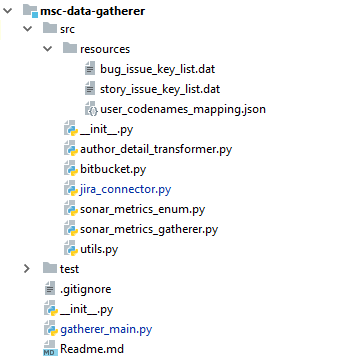
\includegraphics{Figures/impl_src_folder_files.png}
    \caption{Source Files Structure}
    \label{fig:impl-data-gatherer-source-files}
\end{figure}

The source folder structure has been illustrated in Figure \ref{fig:impl-data-gatherer-source-files} and it is comprised of the following elements:
\begin{enumerate}
    \item \texttt{gatherer\_main.py} - included in full in code excerpt \ref{code:gatherer_main.py}. Coordinates all data gathering operations. 
    \item\label{lst:impl.item:jira} \texttt{jira\_connector.py} - Handles all communication and authentication with a given JIRA server.
    \item\label{lst:impl.item:bitbucket} \texttt{bitbucket.py} - handles all communication and authentication with a given Bitbucket server.
    \item\label{lst:impl.item:sonar-metrics-gatherer} \texttt{sonar\_metrics\_gatherer.py} - is responsible for all communication via REST API with Sonar server instance.
    \item\label{lst:impl.item:author-encoder} \texttt{author\_detail\_transformer.py} is responsible for encoding authors' full names into code names to obfuscate sensitive identity details. 
\end{enumerate}

\subsubsection{Operation coordinator - \texttt{gatherer\_main.py}}\label{sec:source-code:main-gatherer}
The starting point of the data gatherer program.

To start with the gatherer program needs to be provided with credentials to JIRA, Bitbucket and Sonar servers that will be contacted in due course. In the current infrastructure, all of those tools were using a the same credentials as they were managed by a single team. Therefore, it is not currently possible to provide different credentials to each tool to be subsequently contacted.

Secondly, should the credentials be omitted the program will notify the user about an error condition and its root cause and then terminate.

The credentials are not immediately validated - each tool handles that separately in their respective classes.

It should also be noted that the program disables any SSL connectivity warnings as SSL validation is skipped during the execution- authentication is carried out using user name and password only.

Subsequently, a list of JIRA keys pertaining to Bug type tickets, described in detail in section \ref{sec:source-code:jira}, are loaded into a list and the execution proper begins.

The order of events is as follows:
\begin{enumerate}
    \item Jira Connector is contacted to obtain a list of files made under each and every JIRA key. Detailed in section \ref{sec:source-code:jira}.
    \item Bitbucket connector is contacted to add information about previous commit made under a given file. Detailed in section \ref{sec:source-code:bitbucket}.
    \item Sonar Connector is contacted to obtain code quality metrics - subject of section \ref{sec:source-code:sonar-metrics}.
    \item an empty CSV, intended to hold the final dataset is created
    \item information obtained from above 3 items is combined into a single object, representing the entirety of the dataset.
    \item column headers are saved - due to the nature of the output from the Sonar connector a special condition had to be implemented to ensure the headers were only saved once per dataset.
    \item the dataset is persisted to the target CSV file
\end{enumerate}

Then, the list of JIRA keys pertaining to the non-bug tickets is loaded into the main component and all of the steps listed above are executed again and all of the information gathered is appended to the CSV representing the final dataset.

It should be noted, that should an error occur at any stage of the execution, it is logged for review. Should an error occur while processing any of the individual files, information about such event, be it in the main component or any of the connectors, is also logged for later review.

\subsubsection{JIRA Connector}\label{sec:source-code:jira}
The very first operation that the JIRA connector class is responsible for is obtaining a list of JIRA keys. Typically composed of 3 to 4 letters, a key is an abbreviation uniquely identifying a given JIRA project. JIRA keys are obtained from a pre-compiled lists: the \texttt{bug\_issue\_key\_list.dat} and \texttt{story\_issue\_key\_list.dat} files, where the former contains only keys to Story-type tickets, while the latter to bug-type tickets. 
All of the communication with JIRA server happens over its publicly available REST API. In order to access it, base URL is required in the form of \mintinline{html}{<server_name>/jira/rest}.

The JIRA connector then interrogates the server by executing \mintinline{html}{/api/2/issue/{jira_key}} in order to obtain an ID attribute for each ticket. Ticket ID is a necessary parameter required in order to obtain the list of files committed under each ticket.

In the next step, a list of commits for a given JIRA ID is obtained for all code repositories from the \mintinline{html}{/dev-status/1.0/issue/detail?issueId={jira_id}&applicationType=stash} URL. The server response is in JSON format and as Figure \ref{fig:source-code:jira:commit-response} illustrates it is possible for any given commit to include multiple files, per repository. Additionally, many commits can be made under the same ticket, under many repositories. Based on Figure \ref{fig:source-code:jira:commit-response}, it should be assumed that the all of the next steps are executed for all files, under any commit in any repository provided by the above REST call.
\begin{figure}[!h]
    \centering
    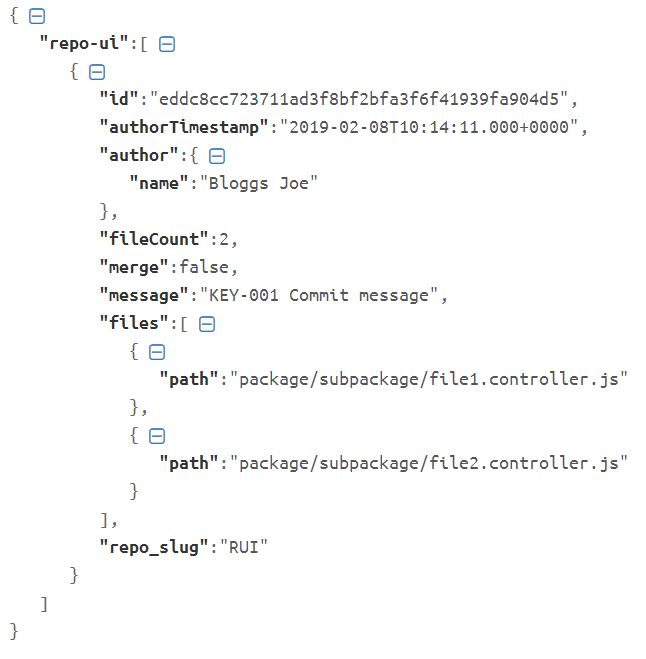
\includegraphics[scale=0.7]{Figures/gatherer/jira_connector_getting_commit_files_response.PNG}
    \caption{Sample Response from JIRA detailing all commits made under given ticket}
    \label{fig:source-code:jira:commit-response}
    
\end{figure}
    
At this step, a number of infrastructure repositories that are maintenance-only, or ones that are written in languages not supported by Sonar server, thus making it impossible to obtain code quality metrics, have been removed. The repository names to be excluded are matched by a regular expression, from a list of static names compiled based on the domain knowledge of the infrastructure present at the business site. The repositories in question were mainly related to testing framework setup and maintenance, deployment pipelines for specific products and applications present at the business site or automated tests, etc. The list is not provided as it includes product names and it has been considered sensitive by the business owners.
    
In the next step, all merge commits are being removed from the analysis as it would otherwise create duplicate data points. For detailed explanation refer to Section \ref{sec:design}. 

Subsequently, a number of files are removed from the analysis - for listing of what file patterns were ignored, refer to Table \ref{tbl:file-extensions-excluded-from-analysis}. The files were excluded by name and/or extension pattern using regular expression and they represented a number of different categories detailed below. 
\begin{table}[!h]
\centering
\caption{Files excluded from the analysis by extension or suffix}
\label{tbl:file-extensions-excluded-from-analysis}
% \begin{tabular}{@{}llll@{}}
% \toprule
% \multicolumn{4}{c}{Exclusion Patterns} \\ \midrule
% .*Test.*.java & .*Interface.*\textbackslash{}.java & .*NameToIndex\textbackslash{}.java & .*\textbackslash{}.jar \\
% .*Test.*.kt & .*Interface.*\textbackslash{}.kt & .*Config.kt & .*Dto.*kt \\
% .*\textbackslash{}.e2e-spec.js & .*\textbackslash{}.stub.js & .*\textbackslash{}.po.js & .*spec.js \\
% .*\textbackslash{}.ico & .*\textbackslash{}.npmrc & .*\textbackslash{}.conf.js & .*gulpfile.js \\
% .*ColumnDef.js & .*Spec.js & .*Decorator.js & \textbackslash{}.eslintrc \\
% .*\textbackslash{}.gitattributes & .*\textbackslash{}.sql & .*\textbackslash{}.csv & .*\textbackslash{}.xlsx \\
% .*\textbackslash{}.txt & .*\textbackslash{}.xlsm & .*\textbackslash{}.yaml & .*\textbackslash{}.yml \\
% .*WriteService.* & .*DeleteService.* & .*CreateService.* & .*\textbackslash{}.lock \\
% .*.gradle & .*\textbackslash{}.?factory.js & .*\textbackslash{}.css & .*.config.js \\
% .*Config.java & .*\textbackslash{}.html & .*\textbackslash{}.svg & .*ColumnDefs.js \\
% .*\textbackslash{}.gz & .*ReadService.* & \textbackslash{}.gitignore & .*\textbackslash{}.json \\
% .*\textbackslash{}.war & .*Enum.*kt & .*\textbackslash{}.scss & .*factories.js \\
% .*Jenkinsfile.* & .*\textbackslash{}.xml & .*\textbackslash{}.md & .*\textbackslash{}.properties \\ \bottomrule
% \end{tabular}

\begin{tabular}{@{}lllll@{}}
\toprule
Test Files & \begin{tabular}[c]{@{}l@{}}Build and Deployment \\ infrastructure\end{tabular} & \begin{tabular}[c]{@{}l@{}}Interfaces, Enums \\ and Transfer Objects\end{tabular} & Project configuration & Other \\ \midrule
.*Test.*.java & .*\textbackslash{}.war & .*Interface.*\textbackslash{}.java & .*Config.java & .*\textbackslash{}.csv \\
.*Test.*.kt & .*Jenkinsfile.* & .*Interface.*\textbackslash{}.kt & .*Config.kt & .*\textbackslash{}.css \\
.*\textbackslash{}.e2e-spec.js & .*\textbackslash{}.jar & .*ReadService.* & .*.config.js & .*\textbackslash{}.svg \\
.*\textbackslash{}.stub.js & .*\textbackslash{}.npmrc & .*Enum.*kt & .*.gradle & .*\textbackslash{}.scss \\
.*Spec.js & .*\textbackslash{}.yml & .*NameToIndex\textbackslash{}.java & \textbackslash{}.gitignore & .*\textbackslash{}.md \\
.*\textbackslash{}.?factory.js & .*\textbackslash{}.lock & .*CreateService.* & .*\textbackslash{}.gitattributes & .*\textbackslash{}.json \\
.*\textbackslash{}.po.js & .*gulpfile.js & .*WriteService.* & .*\textbackslash{}.properties & .*\textbackslash{}.xlsx \\
.*spec.js & \textbackslash{}.eslintrc & .*DeleteService.* &  & .*\textbackslash{}.ico \\
.*ColumnDefs.js & .*\textbackslash{}.conf.js & .*Dto.*kt &  & .*\textbackslash{}.txt \\
.*factories.js & .*\textbackslash{}.yaml & .*Decorator.js &  & .*\textbackslash{}.gz \\
.*ColumnDef.js &  &  &  & .*\textbackslash{}.sql \\
 &  &  &  & .*\textbackslash{}.xlsm \\
 &  &  &  & .*\textbackslash{}.html \\
 &  &  &  & .*\textbackslash{}.xml \\ \bottomrule
\end{tabular}
\end{table}
Firstly, "Test Files" column included the actual test classes housing the automated test scripts, their corresponding fixtures and object factories and any test configuration required by a given project.

The "Build and Infrastructure" column describes any files required, utilized or produced as part of a given project's build and publishing lifecycle. It also included any files relating to the infrastructure as code, which is heavily utilized in the applications under analysis to codify setup of any given deployment.

The third column, "Interfaces, Enums and Transfer Objects", details patterns for specific source code file for which code coverage doesn't exists as they're not strictly executable. This includes Java or Kotlin interface files, which as they do not have a specific file name associated with them, had to be compiled by trial and error and from own domain knowledge. Additionally, all of the enumerations in Java and Kotlin languages were excluded by utilizing the commonly applied "Enum" suffix. Furthermore, all data transfer object, which in the context of applications under analysis would only contain mutator methods, were excluded by utilizing the "Dto" suffix. 

The "Project Configuration" column refers to any configuration files contained in the project, which can refer to both application object setup, in the form of for example Spring Framework's Beans, as well as build tool files and properties. 
The "Other" column contains all of the files that did not fit any of the above categories. It represents the readme files, database scripts and other setup files.

To reiterate, all of the file patterns included in Table \ref{tbl:file-extensions-excluded-from-analysis} represent files for which no source code metrics could presently, be obtained from Sonar server. Therefore, they were removed to prevent generating noise in the analysis.
    
In the next and final step a list of initial metrics identifying a given commit is compiled. Alongside it, a map containing \texttt{issue\_key}, \texttt{source\_repository}, \texttt{commitId}, \texttt{path} and \texttt{repo\_code}, which is a unique 3-4 character abbreviation identifying a repository, however, different that that of JIRA key, is composed. The complete map containing both commit details as well as information necessary in the subsequent step is returned back to the coordinator file. 
    
For code listing for this step refer to code excerpt \ref{code:jira-connector.py}

\subsubsection{Bitbucket Connector}\label{sec:source-code:bitbucket}
The data provided by JIRA server as described in section \ref{sec:source-code:jira} is necessary to communicate with the Bitbucket server over REST API. The role of Bitbucket is to provide details of the previous commit made on a given file, such as its author and timestamp. 

The interrogation as is the case with JIRA, happens over public REST API provided by Bitbucket server by making a call to 
\begin{minted}[breaklines]{html}
<server_name>/rest/api/1.0/projects/{repo_code}/repos/{repo_name}/commits/{commit_id}
\end{minted} 
URL.
The response is given in JSON format and as per Figure \ref{fig:source-code:bitbucket-prev-commit-response} it contains only 4 relevant properties per given commit made on a given file.

\begin{figure}[!h]
    \centering
    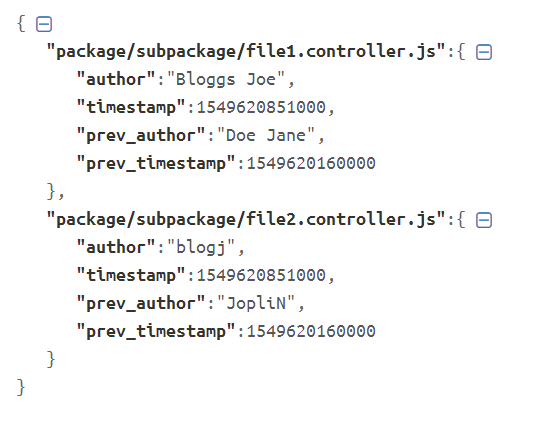
\includegraphics[scale=0.7]{Figures/gatherer/bitbucket_commit_details.PNG}
    \caption{Caption}
    \label{fig:source-code:bitbucket-prev-commit-response}
\end{figure}

As previously described in Section \ref{sec:design}, List \ref{lst:design:info-from-bitbucket} the details listed in Figure \ref{fig:source-code:bitbucket-prev-commit-response} will be used in subsequent analysis steps to provide an indication of developers' level of experience based on seniority as well as familiarity with a given product based on the amount of time spent on the project.
    
In the final step above details, are compiled into a map of arrays, with the a given file name as a key and author and timestamp details as properties inside the array object. The compiled data is then returned to the coordinator script for further processing.

Complete code listing is available from code excerpt \ref{code:bitbucket.py}.
 
\subsubsection{Sonar Metrics Gatherer}\label{sec:source-code:sonar-metrics}
Using data gathered from JIRA and Bitbucket in sections \ref{sec:source-code:jira} and \ref{sec:source-code:bitbucket} Sonar server is contacted for each and every file, for each and every commit under each JIRA ticket. 

In order to retrieve any metrics from Sonar server first a property called a key needs to be obtained. Initially it was attempted to dynamically generate the project key from data already at hand, however, Sonar server doesn't display any easily identifiable pattern in generating its project keys. Instead, a call to, a now deprecated but still functioning REST endpoint, has been made over the publicly available API. 
The call is always made to \mintinline{html}{<server_name>/api/projects/index?search=<project_name>\%20<default_branch>}, and while the "server\_name" and "project\_name" properties are easily obtainable and static in nature, the "default\_branch" property can be different per project basis and depends solely on the setup of a given Bitbucket repository. Currently, in the gathered data only 2 default branches have been detected: "develop" and "master", however, there is a possibility that additional branch names could be present in different data. In general, "master" branch has been used in JavaScript projects and "develop" has been used as a default for Java and Kotlin based repositories. However, given that this is just an observation and it does not carry 100\% certainty, for each project key to be retrieved using above endpoint, both eventualities had to be checked. 

Curiously, the response in this case was returned in XML format and not JSON, which meant that an additional method of parsing out the data had to be devised. 
The easiest solution has been selected, where the XML response in question was automatically converted to a JSON representation. 

When project-key has successfully been obtained it needs to be combined with the name of the repository a given file is in in order to obtain a Sonar component-key. The component-key is part of the request URL made to the Sonar server in order to finally obtain code quality metrics. Without it, there is no avenue to identify which metrics are for which file, in what repository.

The difficulty again, is the lack of overarching consistency in how component-keys are generated when Sonar analysis is first setup as the format has been discovered to differ between JavaScript based project and those written in Java or Kotlin.

To give an example, for JavaScript based projects the component-key format would be:
\texttt{component:branch:module\_name} but for the JVM based languages, like Java, the format is
\texttt{component:module\_name:branch}.
Notice how \texttt{module\_name} and \texttt{branch} switch their positions between languages.
This difference is significant as it allows for forming a hypothesis, that the component-key format may be different yet again for projects in languages that have not been taken into the account so far, for example C\# or Python.
Lastly, the complete component-key is encoded in URL-friendly format.

The final step executed by Sonar gatherer class is to obtain the code quality metrics from the server for each and every file gathered. 

To start with, a target URL is composed from Sonar server address, component key and and a comma-separated list of metrics to be obtained. As part of that operation a specified list of code quality metrics is retrieved. The list is defined in \texttt{sonar\_metrics\_enum.py} and it is comprised of 66 different values, 7 of which are not representing Sonar metrics, but information gathered from other sources, i.e. author, timestamp, etc. 

The response from Sonar server, this time in JSON format, is parsed, and sorted. It should be noted, and it will be discussed in due course, that not all metrics are obtainable for every file gathered. In the instance that a metric is missing, the empty value is replaced with $-1$ as this value, as opposed to $0$ is not a legal value for any code quality metrics. 

One thing of note is that for different source code languages different metrics, especially with regards to the code coverage metrics can be provided by Sonar. For example, for JavaScript-based languages such as Angular JS there is a separate position for integration, or IT, coverage, whereas for Java and other JVM based languages that metric is rarely provided. In JVM based languages it has been folded into the \texttt{overall code coverage} metric instead.

The sorting is performed to ensure that all metrics, which will shortly represent columns in the generated CSV dataset, appear in the same order. Otherwise, it would be quite difficult to execute all subsequent elements of the analysis.

All collected metrics, compiled into a dictionary, where a given file's name is the key and value is represented by metrics is returned to the \texttt{gatherer\_main.py} for persisting.

\subsubsection{Author Detail Transformer}\label{sec:source-code:author-encoder}
It is invoked after code quality metrics have been gathered by \texttt{SonarMetricsGatherer} class. It transforms full names of commit authors into code names. Given that there is no single format of displaying full name in a commit it needed to be robust enough to detect the format of the name. 

Occasionally the commits were not signed with author's full name but their corporate handle, which meant that the transformer had to accommodate those cases as well.

\subsubsection{Other Utilities}
The project contains a utilities file, \texttt{utils.py}, which houses a few functions that are not associated with any given class. It contains 2 functions of note. One is responsible for loading any JSON files from a specified disk location, which is utilized by the \texttt{gatherer\_main.py} author encoding functionality. The second is responsible for cleaning up the empty carriage returns and empty lines in the dataset generated by the Data Gatherer program. 

